We now return to the case study outlined in section \ref{sec:casestudy}. Our surveillance task is $\LTLsquare \LTLdiamond p_5$, i.e, we need to infinitely often bring the belief of the target location to 5 cells or lower. We look at two different partitions of the gridworld in figure \ref{fig:SGR-grid} as shown in figure \ref{fig:bigexp}.

\begin{figure}
\subfloat[The gridworld in \ref{fig:SGR-grid} partitioned into 6 subgames. \label{fig:experiment}]{
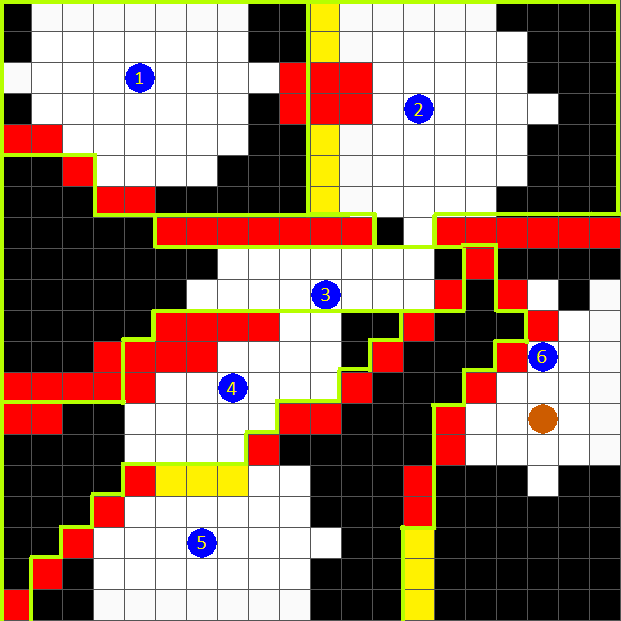
\includegraphics[scale=0.18]{figs/SGR-grid-vis-part.png}
\hspace{.3cm}}
%\hfill
\subfloat[The gridworld in \ref{fig:SGR-grid} partitioned into 3 subgames - one for each mobile sensor. \label{fig:3experiment}]{
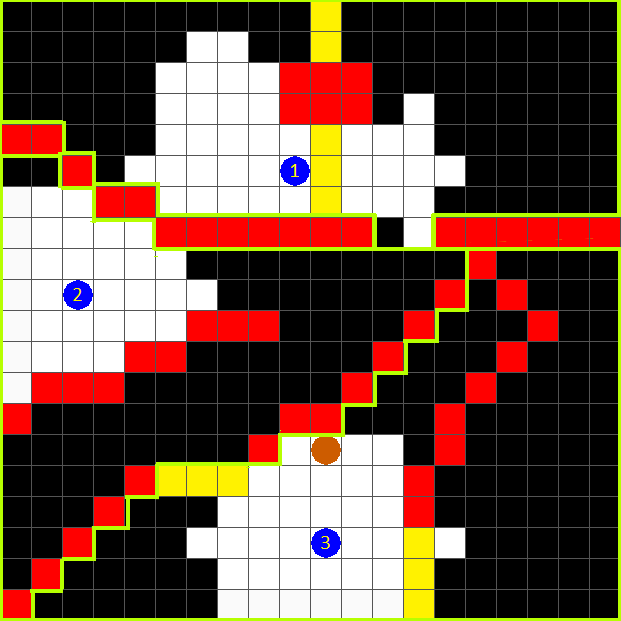
\includegraphics[scale=0.18]{figs/SGR-grid-vis-part_3.png}
\hspace{.3cm}}

\caption{We look at the case where we have 6 mobile sensors in \ref{fig:experiment} and 3 mobile sensors \ref{fig:3experiment}\label{fig:bigexp}}
\end{figure} 

Using this partition, we have 6 subgames. 